\documentclass[12pt, letterpaper]{article}
\usepackage[english]{babel} % Sets the language and regional settings for English documents
\usepackage[utf8]{inputenc} % Allows the use of UTF-8 characters in the document
\usepackage[T1]{fontenc} % Specifies font encoding
\usepackage[margin=2cm]{geometry} % Sets the page margins
\usepackage{makeidx} % Enables the creation of indexes
% \usepackage{natbib} % Provides flexible bibliography support
\usepackage{url} % Allows the use of URLs
\usepackage{enumitem} % Customizes the appearance of lists
\usepackage{listings} % Provides syntax highlighting for code listings
\usepackage[dvipsnames]{xcolor} % Allows the use of colors
\usepackage{parskip} % Modifies paragraph spacing
\usepackage{graphicx} % Enables the inclusion of graphics
\usepackage{tikz} % Allows the creation of graphics and diagrams
\usepackage{float}
\usepackage{hyperref} % Enables the creation of hyperlinks
\usepackage{amsmath} % Provides additional math environments and commands
\usepackage{circuitikz} % Allows the creation of electrical circuits
\usepackage{adjustbox} % Adjusts the size of the circuit diagrams
\usepackage{tcolorbox}
\usepackage{diagbox} % Allows the use of diagonal boxes in table cells
\usepackage{colortbl} % Allows coloring of table cells
\hypersetup{
    colorlinks=true,
    linkcolor=blue,
    urlcolor=blue
}
\usepackage{breakurl} % Allows links to break across lines
\definecolor{mygray}{gray}{0.9}

\usetikzlibrary{shapes.geometric, positioning}

\lstset{
    language=SQL,
    basicstyle=\ttfamily\small,
    keywordstyle=\color{blue},
    commentstyle=\color[rgb]{0,0.5,0},
    stringstyle=\color{red},
    numbers=left,
    numberstyle=\tiny\color{gray},
    stepnumber=1,
    numbersep=10pt,
    backgroundcolor=\color{white},
    showspaces=false,
    showstringspaces=false,
    breaklines=true,
    frame=single,
    tabsize=2, captionpos=b, lineskip=-1pt,
    extendedchars=true,
    literate={á}{{\'a}}1 {é}{{\'e}}1 {í}{{\'i}}1 {ó}{{\'o}}1 {ú}{{\'u}}1 {Á}{{\'A}}1 {É}{{\'E}}1 {Í}{{\'I}}1 {Ó}{{\'O}}1 {Ú}{{\'U}}1 {ñ}{{\~n}}1 {Ñ}{{\~N}}1 {¿}{{\textquestiondown}}1 {¡}{{\textexclamdown}}1
}

% VHDL language configuration
\lstdefinelanguage{VHDL}{
    morekeywords={entity, architecture, signal, port, in, out, inout, begin, end, process, if, then, else, elsif, case, when, others, for, while, loop, wait, library, use, std_logic, std_logic_vector, integer, boolean, rising_edge, falling_edge, component, generic, map, downto, to, and, or, not, xor, nand, nor, xnor},
    morecomment=[l]{--},
    morestring=[b]",
    sensitive=false,
    alsoletter={_}
}

% VHDL listings style at the same time that there is 
\lstdefinestyle{vhdl}{
    language=VHDL,
    basicstyle=\ttfamily\small,
    keywordstyle=\color{blue}\bfseries,
    commentstyle=\color[rgb]{0,0.6,0}\itshape,
    stringstyle=\color{red},
    numbers=left,
    numberstyle=\tiny\color{gray},
    stepnumber=1,
    numbersep=10pt,
    backgroundcolor=\color{white},
    showspaces=false,
    showstringspaces=false,
    breaklines=true,
    frame=single,
    tabsize=2,
    captionpos=b,
    lineskip=-1pt,
    extendedchars=true
}

\graphicspath{ {./img/} } % Sets the path for the graphics

\newlist{biblio}{enumerate}{1}
\setlist[biblio,1]{label=[\arabic*]}

\makeindex

\begin{document}

\begin{titlepage}

    \begin{tikzpicture}[remember picture,overlay]
        \node[anchor=north, inner sep=30] at (current page.north) {
            
\includegraphics[width=4.5cm]{logo-cuadrado-transparente.png} % Uncomment if you have the image
        };
    \end{tikzpicture}

    \begin{center}
        \vspace*{4cm}

        \Huge
        \textbf{Proposal: SwayLayoutManager}\\

        \vspace{2.5cm}

        \Huge
        Laboratorio de Investigación y Desarrollo de Software Libre (LIDSoL)\\

        \vspace{2.5cm}

        % Target areas
        \begin{center}
        \textbf{Areas:}\\
        \vspace{0.5em}
        Frontend\\
        Backend
        \end{center}

        \vspace{2.5cm}

        \Huge
        % Proposal date
        \textbf{Date:} September 23, 2025\\
        \vspace{2.5cm}
    \end{center}
\end{titlepage}

\newpage

\section*{Project Title}
SwayLayoutManager: Workspace Layout Manager

\section*{Detailed Description}
\subsection*{Problem}

Users of \textbf{\texttt{--Sway Window Manager--}} often organize their applications into specific layouts across multiple workspaces to optimize their workflow. Reopening every app manually and arranging them can be time consuming and tedious.

\subsection*{Proposed Solution}

The idea behind \textbf{SwayLayoutManager} is to create a versatile application that automates this process through two distinct interfaces: a \textbf{command-line interface (CLI)}, perfect for scripting and automation, and an intuitive \textbf{graphical user interface (GUI)} for easy visual management. Through either interface, users can save the current window layout (applications, arrangement, and workspace) as a named "template" or "preset." Subsequently, they can load this template via \textbf{CLI} with a sway short-cut or through the \textbf{GUI} app to instantly restore all applications to their designated positions and workspaces.

\subsection*{Use Case}
A developer might have a workspace with a \textit{Visual Studio Code} window occupying the left half of the screen and two \texttt{foot} terminals stacked vertically on the right half. With \texttt{SwayLayoutManager}, they could save this layout as \texttt{dev-workspace}. When starting their computer, they could run a simple command to load this template and have their development environment ready instantly, without needing to open and position each window manually.

\begin{figure}[H]
    \centering
    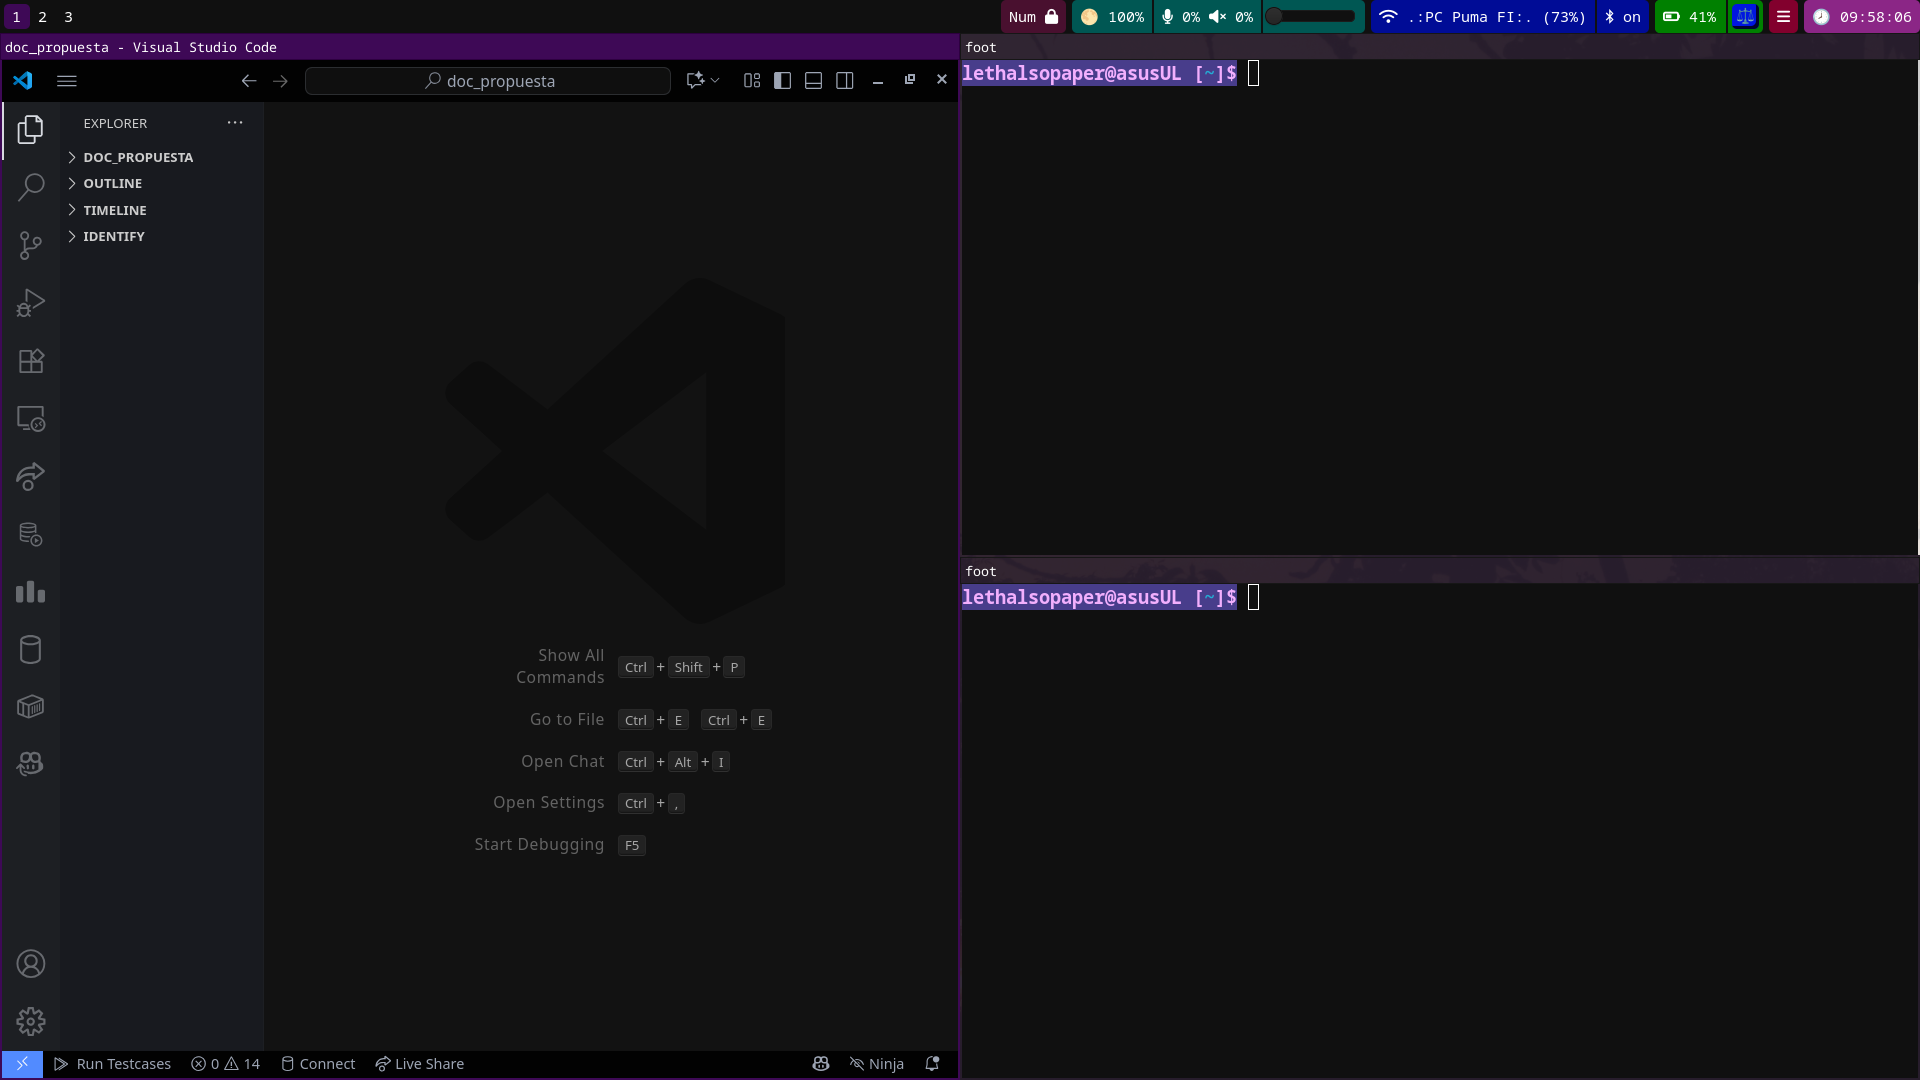
\includegraphics[width=0.8\textwidth]{usea_case_1.png}
    \caption{Use case}
\end{figure}

\section*{Requirements}
\begin{itemize}
    \item \textbf{Operating System:} Any GNU/Linux distribution with \textbf{Wayland} support.
    \item \textbf{Window Manager:} \texttt{sway} (version 1.10 or higher).
    \item \textbf{Core CLI (Backend):}
    \begin{itemize}
        \item Developed in \textbf{Go}, compiling to a single executable.
        \item Has \textbf{no runtime dependencies} for the end-user.
    \end{itemize}
    \item \textbf{GUI (Frontend):}
    \begin{itemize}
        \item Developed in \textbf{Python 3}.
        \item Requires a Python 3 interpreter and a GUI toolkit library (e.g., PyQt6, Tkinter) to run.
    \end{itemize}
    \item \textbf{User Knowledge:} Familiarity with the Linux terminal and basic \texttt{sway} configuration concepts.
\end{itemize}

\section*{Implementation Details}

\subsection*{Internal Operation}

The tool will interact directly with the \texttt{sway} process via swaymsg utility which communicates to the IPC (\textit{Inter-Process Communication}) socket, which allows querying the window manager's state and sending it commands programmatically.

\subsubsection*{Saving Templates (\texttt{save})}
\begin{enumerate}
    \item The command \texttt{swaymsg -t get\_tree} will be executed to get a full JSON dump of \texttt{sway}'s current layout tree.
    \item The application will parse this JSON to extract relevant information for each window in the specified workspaces: the application identifier (\texttt{app\_id} or \texttt{window\_class}), the workspace it belongs to, its layout (horizontal/vertical), and its relative position in the container.
    \item This structured information will be saved to a readable configuration file, for example, \texttt{\~{}/.config/swaylayoutmanager/presets/template\_name.json}.
\end{enumerate}

\subsubsection*{Loading Templates (\texttt{load})}
\begin{enumerate}
    \item The tool will read the configuration file for the template specified by the user.
    \item It will iterate over each application defined in the template.
    \item For each application, it will execute a sequence of \texttt{swaymsg} commands to recreate the layout. This includes:
    \begin{itemize}
        \item Switching to the correct workspace (\texttt{swaymsg workspace number <N>}).
        \item Launching the application (\texttt{swaymsg exec <command>}) if it is not already running.
        \item Using \texttt{sway}'s selection criteria (e.g., \texttt{[app\_id="..."]}) to focus the newly opened window and move or adjust it to the saved layout.
    \end{itemize}
\end{enumerate}

\subsection*{User Interface (CLI)}

The main interaction will be through the terminal, with this subcommand structure:

\subsubsection*{\texttt{swaylayoutmgr save <name>}}

Captures the current state of all active workspaces and saves it as a named layout preset. The command executes \texttt{swaymsg -t get\_tree | jq} to extract workspace layouts, window positions, application identifiers and some other relevant information.

This data is saved into a JSON file wich will be located in \texttt{\~{}/.config/swaylayoutmanager/presets/<name>.json} with metadata for future restoration.

\subsubsection*{\texttt{swaylayoutmgr load <name>}}

Reads a saved preset and recreates the workspace layout by launching applications and positioning them according to the saved configuration. The process involves:

\begin{enumerate}
    \item Parsing the preset JSON and validating its structure
    \item Switching to each workspace and optionally clearing existing windows
    \item Launching missing applications using \texttt{swaymsg exec <command>}
    \item Applying layout reconstruction through \texttt{swaymsg} commands for positioning, resizing, and focus restoration
    \item Handling errors gracefully by skipping unavailable applications and logging issues
\end{enumerate}

\subsubsection*{\texttt{swaylayoutmgr list}}

Displays all available presets with or without metadata including creation date, workspace count, and application summary. The command scans \texttt{\~{}/.config/swaylayoutmanager/presets/} for JSON files and validates their integrity and compatibility.

\textbf{Example Output:}

\begin{lstlisting}[language=bash, caption=Layout preset list output]
Available Layout Presets:
  dev-workspace      (3 workspaces, 5 apps)    [Valid]
    Created: 2024-12-15 14:30

  media-setup        (2 workspaces, 3 apps)    [Valid]
    Created: 2024-12-10 09:15

  presentation-mode  (1 workspace, 2 apps)     [Invalid - missing app]
    Created: 2024-12-01 16:45
\end{lstlisting}

\subsubsection*{\texttt{swaylayoutmgr delete <name>}}

Removes a saved preset after user confirmation. Includes \texttt{--force} flag for scripting and \texttt{--backup} flag for safety.

\end{document}